%Preambulo
\documentclass[a0paper]{tikzposter}
\usepackage[spanish]{babel}
\usepackage[utf8]{inputenc}
\usepackage{amsmath}
\usepackage{blindtext}
\usepackage{graphicx}

\usecolorstyle{Russia}
\usetitlestyle{VerticalShading}
\usebackgroundstyle{Rays}
\usecolorstyle[colorPalette=BlueGrayOrange]{Default}

\title{\parbox{\linewidth}{\centering Investigación de Estrategias de Obtención de Mediciones EIT para Rastreo de Dispersión de líquidos.}}
\author{Osben F. Cándido-Sánchez}
\institute{Departamento de Ingeniería Electrónica, Instituto Tecnológico de Morelia}

\titlegraphic{
\includegraphics[width=8.5in]{logo-sep.png} \quad   
\includegraphics[width=3in]{Itmorelia.png} 
\includegraphics[width=6.5in]{logo-tecnm.png}}

\begin{document}
  \maketitle
  \block{Introducción}{
En la última década, la tomografía de impedancia eléctrica (Electrical Impedance Tomography: \textit{EIT}) ha recibido considerable atención por parte de la comunidad científica en el mundo para aplicaciones médicas e industriales. En medicina, EIT es una herramienta que puede ser aplicable para rastrear la difusion de medicamentos quimioterapeúticos para tratamiento de cáncer de mama \cite{Gnecchi2018}. El estudio de cáncer de mama por EIT está aprobado por la FDA para ayudar a clasificar los tumores encontrados en los mamogramas. Sin embargo, hasta el momento no se han realizado suficientes pruebas clínicas para que se pueda usar en pruebas de detección del cáncer de seno \cite{Cancer.org}.La EIT podría usarse como complemento de la mamografía y la ecografía para la detección del cáncer de mama. Sin embargo, la diferenciación de las lesiones malignas de las benignas en función de las mediciones de impedancia requiere más investigación\cite{Zou2003}.\\
En general, el objetivo de la \textit{EIT} es el de reconstruir imágenes, las cuales representan una sección transversal de una distribucion espacial de impedancia eléctrica interna de un objeto, ya sea en dos o tres dimensiones \cite{Mendoza2012}.\\
Este trabajo está dedicado a proponer una metodología para obtener, reconstruir y analizar mediciones EIT que permitan proponer modelos matemáticos de procesos que involucren la dispersión de líquidos en medios permeables.\\}
\block{Metodología}{
La tomografía de impedancia eléctrica se basa en una número de electrodos unidos a la periferia del objeto para ser estudiado,a diferencia de la tomografía de rayos X, donde las placas de excitación y detección pueden girar alrededor del objeto. En EIT los electrodos se fijan equidistantemente alrededor del objeto, en general, una señal de voltaje es generada, la señal de voltaje se convierte en corriente a través de un VCCS (fuente de corriente controlada por voltaje) y pasa a través de un arreglo multiplexor. El conjunto multiplexor selecciona qué pares de electrodos se utilizan para la corriente.
\begin{tikzfigure}
  \label{fig:MyFigure}
  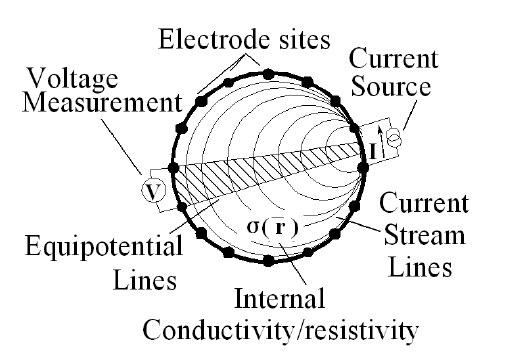
\includegraphics[width=8in]{imagen1.png}
\end{tikzfigure}
}
\begin{columns}
  \column{.50}
  \block{Más ejemplos de LaTeX}{}

  \column{.50}
  \block{Hipotesis}{}

\end{columns}
\block{Referencias}{
\bibliographystyle{IEEEtran}
\bibliography{bibliography}}
\end{document}
